% Insert before \end{document}; copy figures/ beside the main .tex file.
\section{Resultados}

\begin{frame}{Configuração do segundo experimento}
\centering
\large $3 \rightarrow 32 \rightarrow 32 \rightarrow 32 \rightarrow 2$

\medskip
\normalsize Tanh \quad Adam: $\eta=10^{-3}$ \quad Pesos adaptativos: CI, CC e EDP

\bigskip
\begin{tabular}{lrr}
\toprule
& PINN & PINN-DE \\
\midrule
Indivíduos DE & --- & 32 \\
Gerações DE & --- & 100 \\
Avaliações DE & 0 & 3.232 \\
Passos Adam & 8.064 & 4.832 \\
Avaliações de treino & 8.064 & 8.064 \\
\bottomrule
\end{tabular}

\bigskip
3 sementes por método: 2028, 2029 e 2030. Treino em lote completo.

\smallskip
\footnotesize Mesmo número de avaliações; custos distintos por avaliação.
\end{frame}

\begin{frame}{Problema efetivamente utilizado nos testes}
\begin{align*}
u_t+(u^2/2)_x+(uv)_y &= \nu(u_{xx}+u_{yy}),\\
v_t+(uv)_x+(v^2/2)_y &= \nu(v_{xx}+v_{yy}).
\end{align*}
\[
u(0,x,y)=0{,}5+\sin(2\pi x/1{,}5)\cos(2\pi y/1{,}5)
\]
\[
v(0,x,y)=0{,}25-\cos(2\pi x/1{,}5)\sin(2\pi y/1{,}5)
\]
\centering
$\nu=0{,}01$ \quad $(x,y)\in[0;1{,}5]^2$ \quad $t\in[0,1]$

\medskip
$\partial_n u=\partial_n v=0$ nas quatro faces.
\end{frame}

\begin{frame}{Avaliação fora dos pontos de treino}
\centering
\begin{tabular}{lc}
\toprule
Referência & FVM: $h=0{,}05$, $k=0{,}005$ \\
Validação & 45.000 pontos \\
Teste & 45.000 pontos, separados da validação \\
Resíduo da EDP & 4.725 pontos independentes \\
Condição inicial & 900 pontos \\
\bottomrule
\end{tabular}

\bigskip
\[
\mathrm{RMSE}=\sqrt{\frac{1}{2N}\sum_{j=1}^{N}
\left[(u_j-u_j^{\mathrm{FVM}})^2+(v_j-v_j^{\mathrm{FVM}})^2\right]}
\]
\medskip
\footnotesize Referência numérica aproximada; conjunto de teste já inspecionado anteriormente.
\end{frame}

\begin{frame}{Precisão: média e desvio-padrão}
\centering
\normalsize
\begin{tabular}{lcc}
\toprule
RMSE $\downarrow$ & PINN & PINN-DE \\
\midrule
Validação & $0.3176 \pm 0.0149$ & $0.2550 \pm 0.0100$ \\
Teste & $0.3174 \pm 0.0147$ & $0.2559 \pm 0.0098$ \\
EDP & $0.0308 \pm 0.0062$ & $0.0984 \pm 0.0197$ \\
Condição inicial & $0.3081 \pm 0.0259$ & $0.1698 \pm 0.0317$ \\
\bottomrule
\end{tabular}

\bigskip
\begin{block}{Resultados de três sementes}
PINN-DE: menor erro de teste nas três sementes.\\
PINN: menor resíduo independente da EDP.
\end{block}
\end{frame}

\begin{frame}{Erro de teste ao longo do tempo}
\centering

\includegraphics[width=0.94\linewidth,height=0.72\textheight,keepaspectratio]{figures/test_error_by_time.png}

\small Média $\pm$ desvio-padrão; PINN-DE apresenta menor erro médio nos tempos avaliados.
\end{frame}

\begin{frame}{Condição inicial: comparação dos campos}
\centering
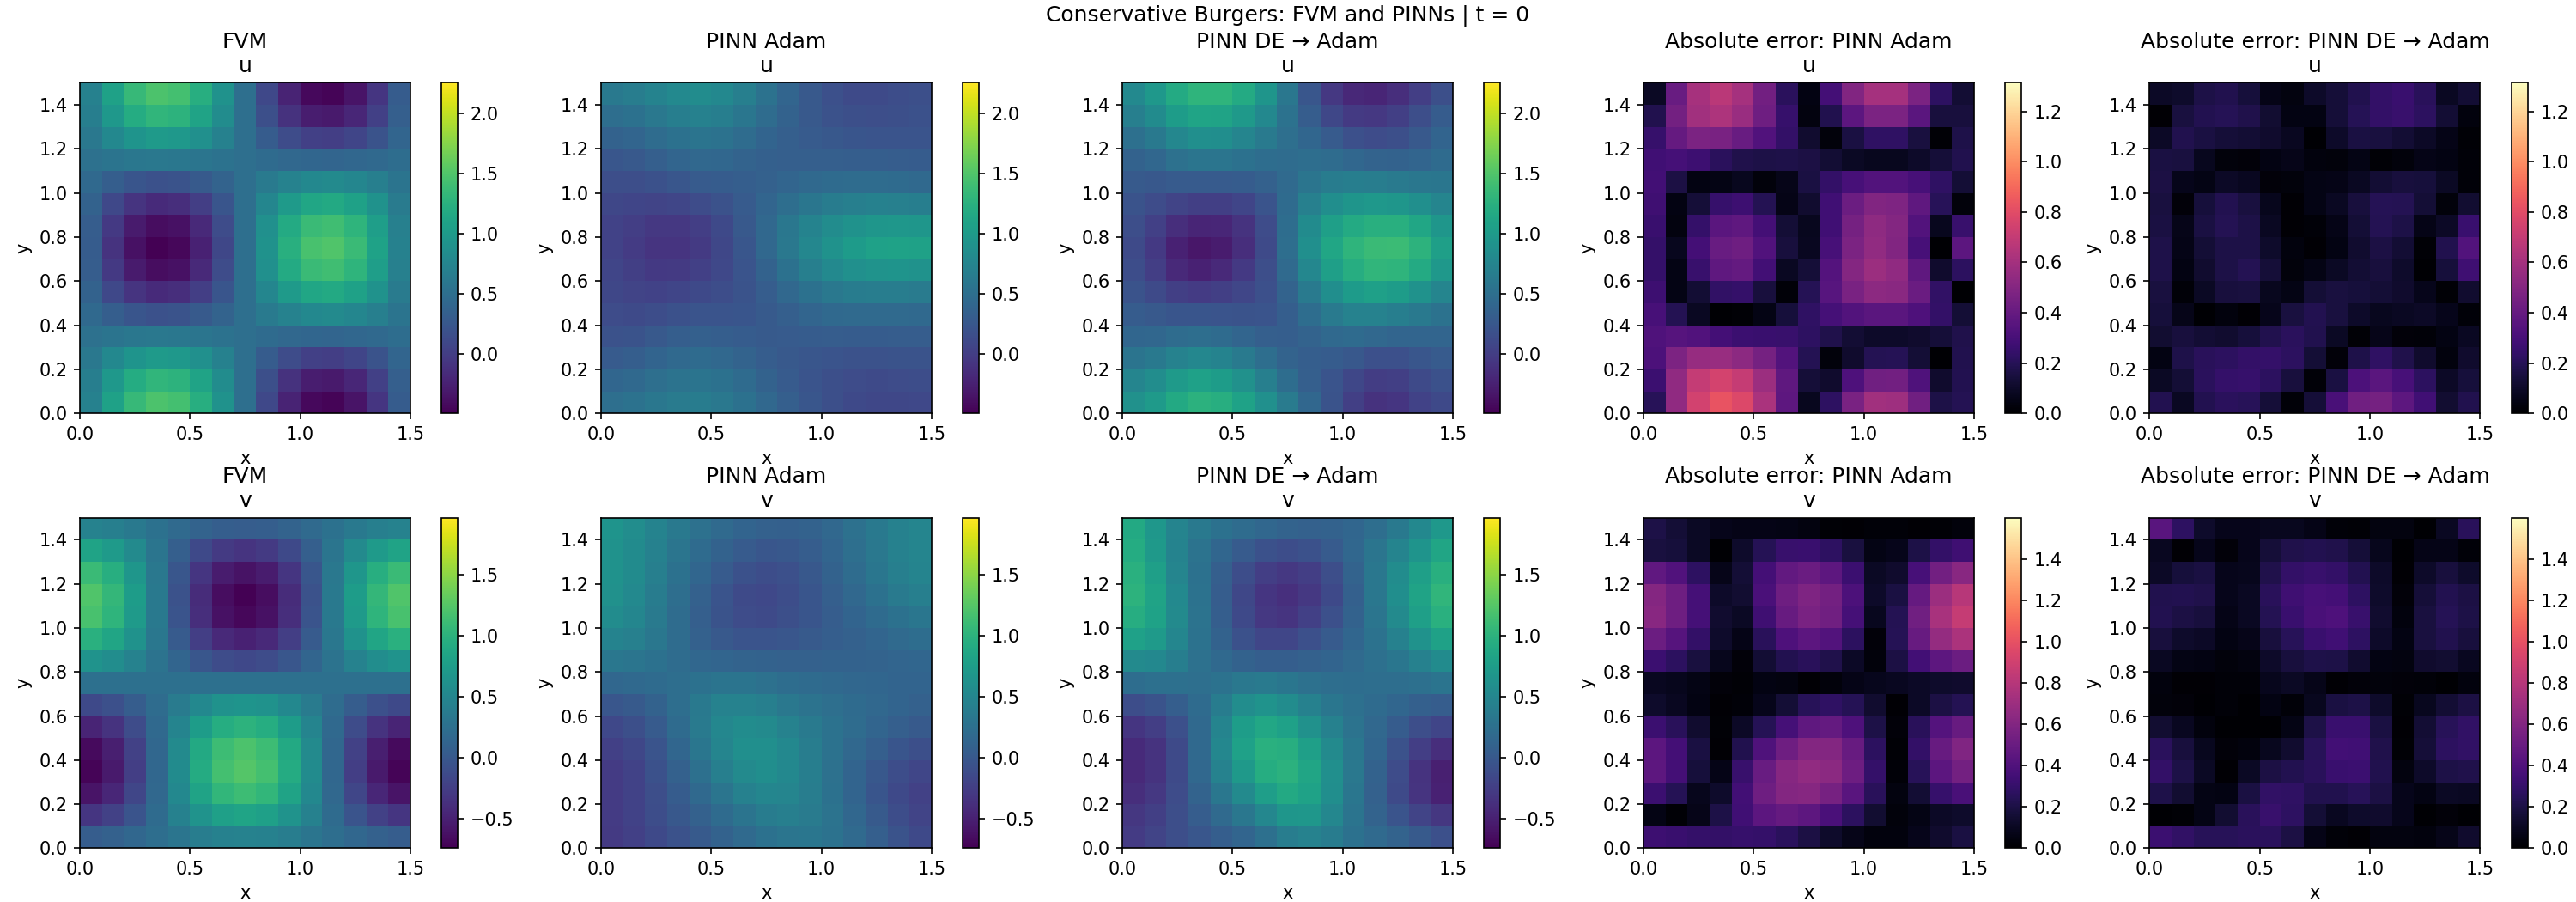
\includegraphics[width=\linewidth,height=0.76\textheight,keepaspectratio]{figures/initial_fields.png}

\footnotesize Semente 2028; FVM com $h=0{,}1$. PINN atenua mais as variações iniciais.
\end{frame}

\begin{frame}{Tempo final: comparação dos campos}
\centering
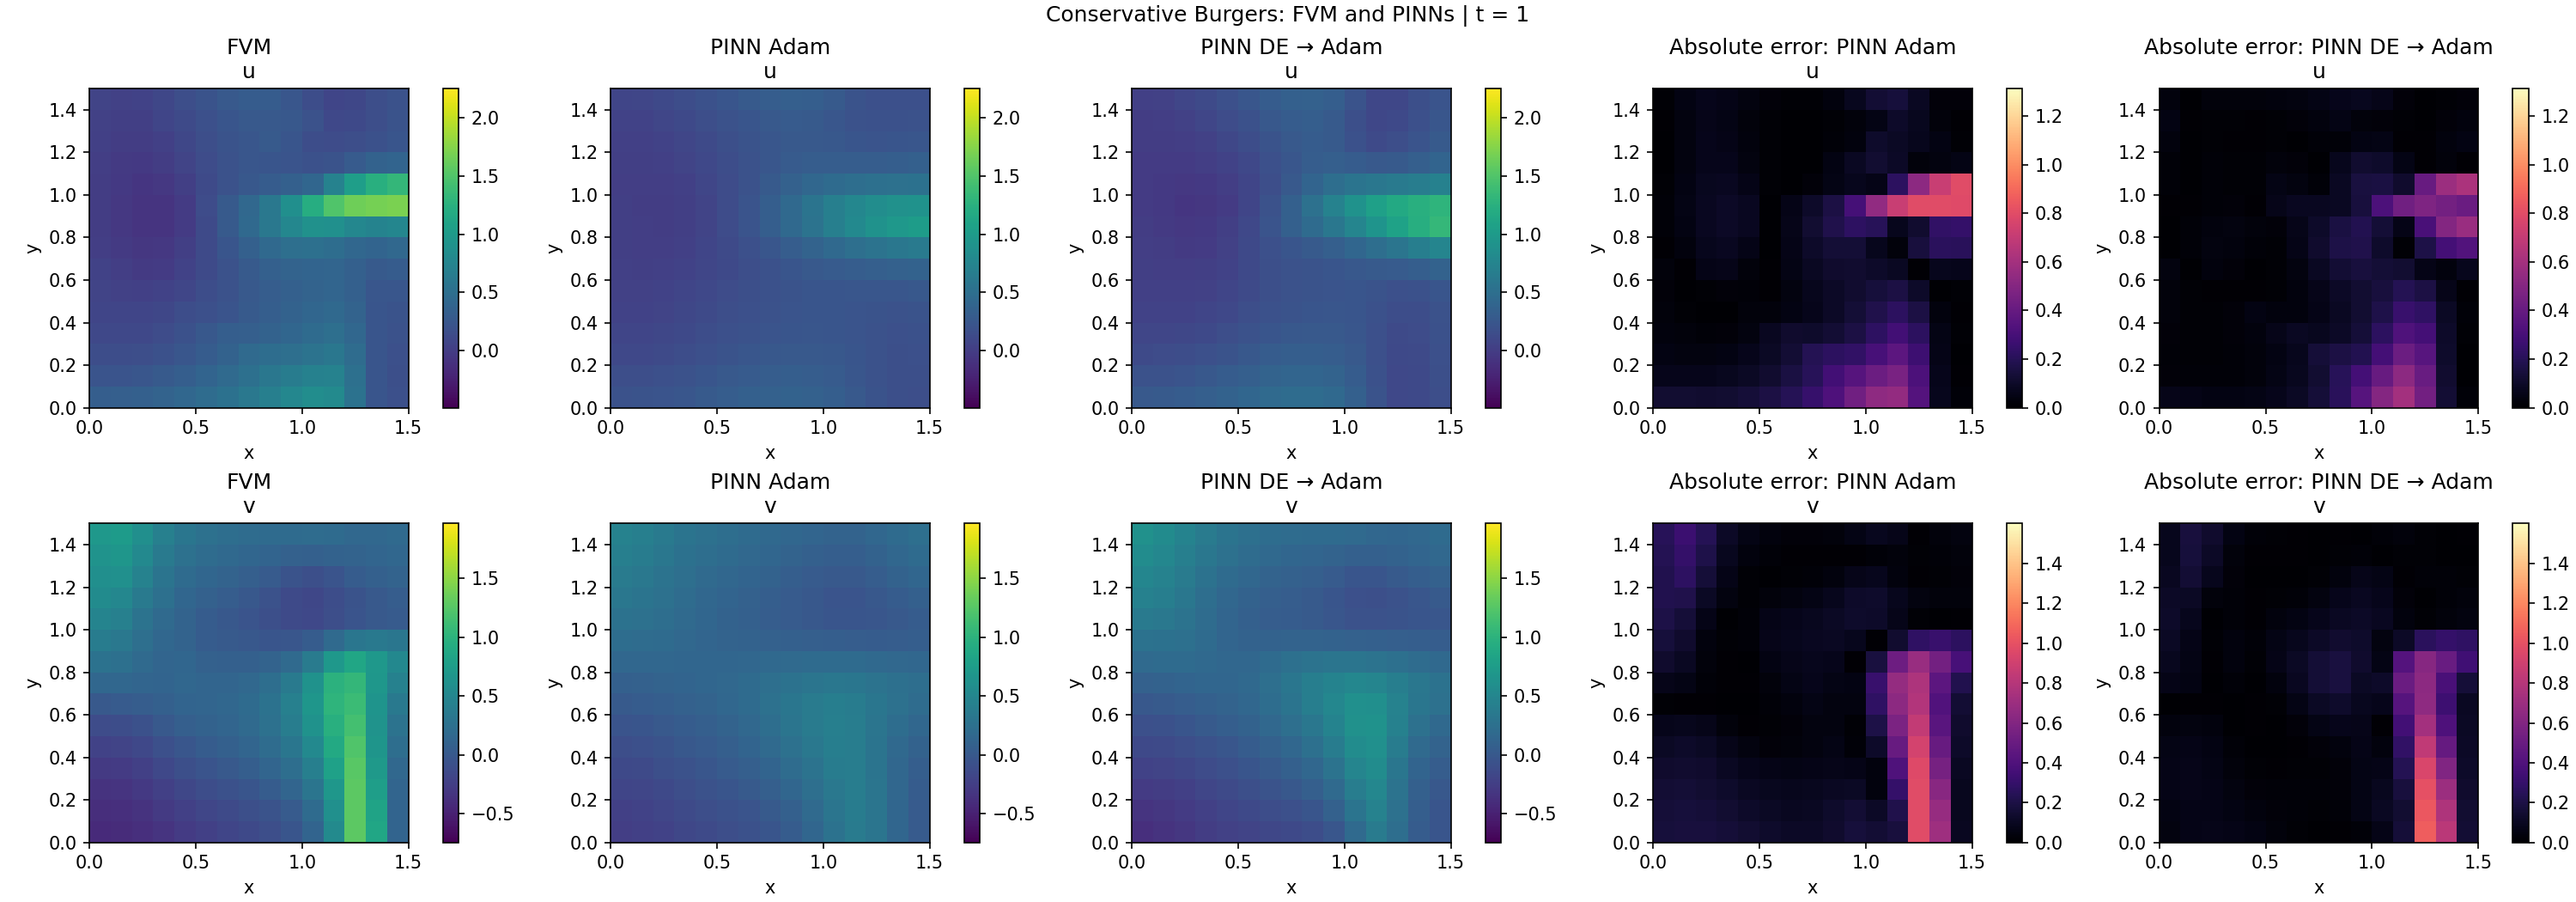
\includegraphics[width=\linewidth,height=0.76\textheight,keepaspectratio]{figures/final_fields.png}

\footnotesize $t=1$; semente 2028; FVM com $h=0{,}1$. Ambos suavizam estruturas do campo.
\end{frame}

\begin{frame}{Evolução das perdas durante Adam}
\centering

\includegraphics[width=\linewidth,height=0.73\textheight,keepaspectratio]{figures/training_losses.png}

\small A perda inicial cresce no fim, enquanto contorno e EDP diminuem.
\end{frame}

\begin{frame}{Convergência da fitness adaptativa no DE}
\centering

\includegraphics[width=0.92\linewidth,height=0.68\textheight,keepaspectratio]{figures/de_convergence.png}

\small $F=\sum_i(e^{-s_i}L_i+s_i)$ \qquad Semente 2028; 32 indivíduos, 100 gerações.
\end{frame}

\begin{frame}{Fitness adaptativa e perda sem pesos}
\centering

\includegraphics[width=\linewidth,height=0.67\textheight,keepaspectratio]{figures/de_diagnostics.png}

\small ``Selected by DE fitness'': $R=L_{\mathrm{CI}}+L_{\mathrm{CC}}+L_{\mathrm{EDP}}$ do vencedor.

\medskip
\alert{A fitness $F$ pode diminuir enquanto a perda sem pesos $R$ aumenta.}
\end{frame}

\begin{frame}{Custo computacional}
\centering
\normalsize
\begin{tabular}{lcc}
\toprule
Tempo (s) & PINN & PINN-DE \\
\midrule
DE & $0.0 \pm 0.0$ & $83.8 \pm 1.5$ \\
Adam & $397.0 \pm 20.0$ & $242.8 \pm 5.2$ \\
Total & $397.0 \pm 20.0$ & $326.6 \pm 3.8$ \\
\bottomrule
\end{tabular}

\bigskip
\begin{block}{Mesmo orçamento de avaliações}
PINN-DE utilizou menos tempo médio de treinamento.
\end{block}
\footnotesize Média $\pm$ desvio-padrão; GTX 1650, float32. Sem tempo de pós-processamento.
\end{frame}

\begin{frame}{Conclusões e limites}
\begin{block}{Observado}
PINN-DE: menor RMSE de teste e da condição inicial.\\[0.15cm]
PINN: menor resíduo da EDP.
\end{block}
\medskip
\begin{alertblock}{Cuidado com o objetivo adaptativo}
Menor fitness não garante menor erro físico.\\[0.15cm]
A perda pode ser ilimitada inferiormente quando um resíduo é zero.
\end{alertblock}
\medskip
\centering
\footnotesize Três sementes; teste reutilizado; convergência da malha FVM não estabelecida.\\
Sem conclusão de significância estatística.
\end{frame}
